\section{Finite Volume Method for the Shallow Water Equations}
In this section, we present the finite volume method (FVM) for solving nonlinear systems of balance laws, specifically focusing on the shallow water equations (SWE).
Nonlinear problems are more challenging than linear problems, as stability and convergence theory are more difficult.
Our focus is on discountinuous solutions, that can accurately capture shock waves and other discontinuities.
The approach described here is based on the work of LeVeque~\cite{LeVeque2002}.

In finite volume methods, the computational domain is discretized into cells or control volumes.
At the interfaces between these cells, we solve the local Riemann problem to compute the fluxes.
These fluxes are then used to update the solution in each cell.
By solving the Riemann problem at cell interfaces, the FVM can handle discontinuous solutions, making it particularly well suited for hyperbolic balance laws, such as the shallow water equations.

\subsection{Finite Volume Methods for the 1D SWE}
We begin by considering finite volume methods for the SWE in one space dimension.
In the FVM, we discretize the domain into finite control volumes or cells:
\begin{align*}
    V_i = [x_{i-1/2}, x_{i+1/2}] \times [t_n, t_{n+1}],
\end{align*}
where $\Delta x = x_{i+1/2} - x_{i-1/2}$ is the length of the cell and $\Delta t = t_{n+1} - t_n$ is the time step.
The cell $V_i^n$ is illustrated in Figure~\ref{fig:control_volume_V_i_n}.
\begin{figure}[H]
    \centering
    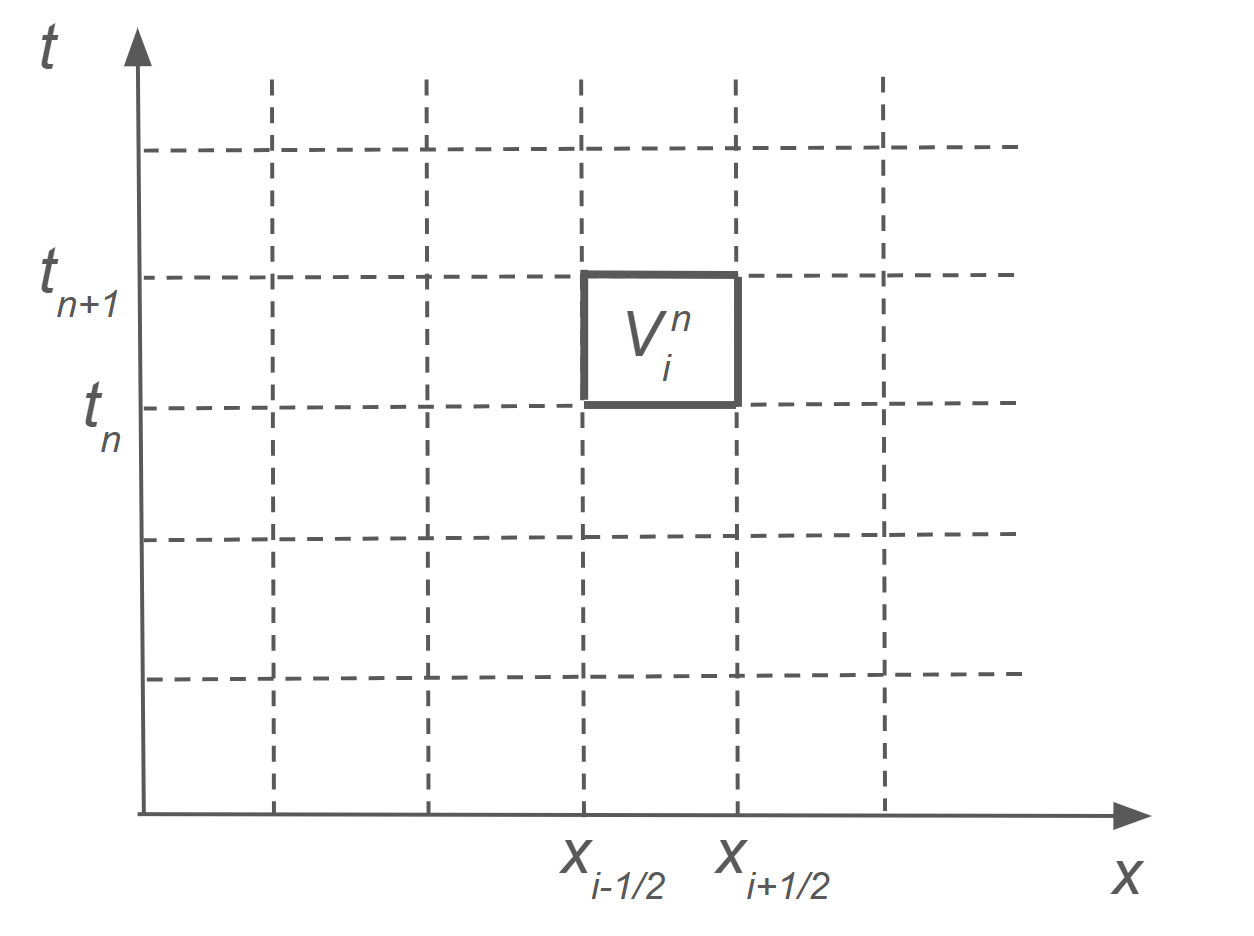
\includegraphics[width=0.4\textwidth]{C:/Users/Matteo/Shallow-Water-Equations/tex/figs/control_volume_V_i_n.png}
    \caption{Illustration of the control volume $V_i^n$ in the $x,t$ plane.}\label{fig:control_volume_V_i_n}
\end{figure}
For now, we will assume a uniform grid for simplicity.
The finite volume formula is derived from the integral form~\eqref{eq:integral_form_1D_final}.
By dividing the integral form of the 1D inhomoegeneous SWE by the cell length $\Delta x$, we espress it in terms of the newly defined cells:
\begin{align*}
    \frac{1}{\Delta x} \int_{x_{i-1/2}}^{x_{i+1/2}} \mathbf{U}(x,t_{n+1}) \text{ d}x &= \frac{1}{\Delta x} \int_{x_{i-1/2}}^{x_{i+1/2}} \mathbf{U}(x,t_n) \text{ d}x\\
    & - \frac{\Delta t}{\Delta x} \left[ \frac{1}{\Delta t} \int_{t_n}^{t_{n+1}} \mathbf{F}(\mathbf{U}(x_{i+1/2}, t)) \text{ d}t
    - \frac{1}{\Delta t} \int_{t_n}^{t_{n+1}} \mathbf{F}(\mathbf{U}(x_{i-1/2}, t)) \text{ d}t \right] \\
    &+ \frac{\Delta t}{\Delta x \Delta t} \int_{x_{i-1/2}}^{x_{i+1/2}} \int_{t_n}^{t_{n+1}} \mathbf{S(U)}(x,t) \text{d}x \text{d}t.
\end{align*}
For a finite volume $V_i^n$, averaging the terms over the volume yields the explicit conservative form
\begin{align}\label{eq:explicit_conservative_1D_SWE}
    \mathbf{U}_i^{n+1} = \mathbf{U}_i^n - \frac{\Delta t}{\Delta x} \left( \mathbf{F}_{i+1/2}^n - \mathbf{F}_{i-1/2}^n \right) + \Delta t \mathbf{S}_i.
\end{align}
The formula~\eqref{eq:explicit_conservative_1D_SWE} is referred to as a finite volume scheme.
The value $\mathbf{U}_i^n$ is the average value over the $i$-th cell at time $t_n$:
\begin{align}
    \mathbf{U}_i^n = \frac{1}{\Delta x} \int_{x_{i-1/2}}^{x_{i+1/2}} \mathbf{U}(x,t_n) \text{ d}x,
\end{align}
also known as the cell average.
The flux $\mathbf{F}_{i-1/2}^n$ is the average flux across the line $x = x_{i-1/2}$ from time $t_n$ to $t_{n+1}$:
\begin{align*}
    \mathbf{F}_{i-1/2}^n = \frac{1}{\Delta t} \int_{t_n}^{t_{n+1}} \mathbf{F}(\mathbf{U}(x_{i-1/2},t)) \text{ d}t,
\end{align*}
and correspondingly the flux $\mathbf{F}_{i+1/2}^n$ is the average flux across the line $x = x_{i+1/2}$ from time $t_n$ to $t_{n+1}$:
\begin{align*}
    \mathbf{F}_{i+1/2}^n = \frac{1}{\Delta t} \int_{t_n}^{t_{n+1}} \mathbf{F}(\mathbf{U}(x_{i+1/2},t)) \text{ d}t.
\end{align*}
The source term $\mathbf{S}_i$ is the average source term over the $i$-th cell at time $t_n$:
\begin{align*}
    \mathbf{S}_i &= \frac{1}{\Delta t \Delta x} \int_{t_n}^{t_{n+1}} \int_{x_{i-1/2}}^{x_{i+1/2}} \mathbf{S}(x,t) \text{ d}x\text{d}t.
\end{align*}
The values are illustrated in Figure~\ref{fig:10_3}.
\begin{figure}[H]
    \centering
    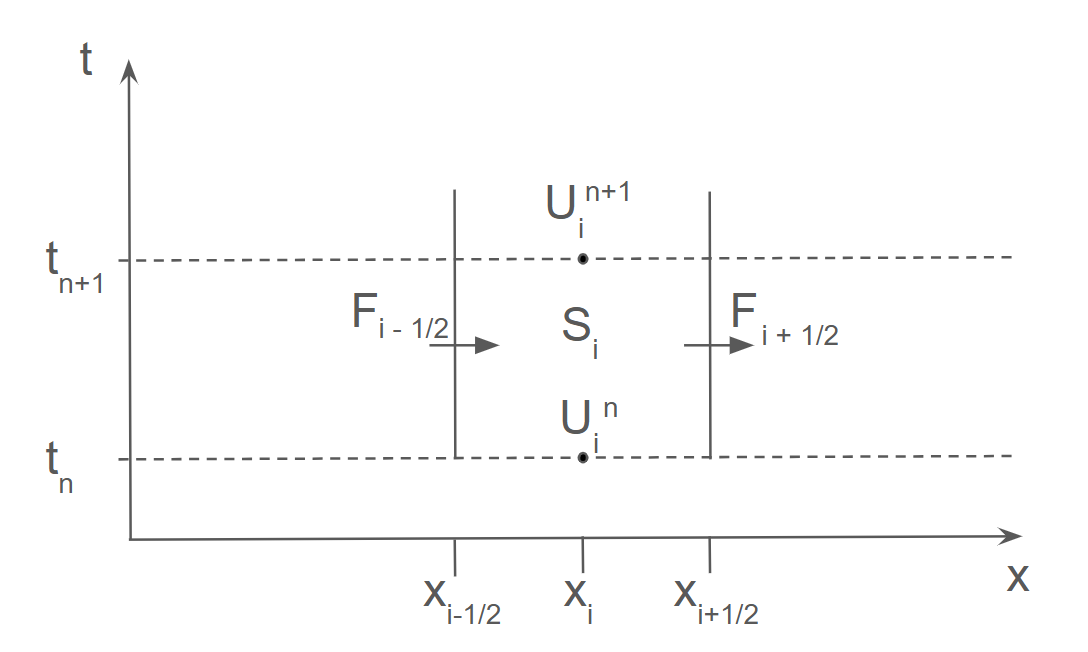
\includegraphics[width=0.5\textwidth]{C:/Users/Matteo/Shallow-Water-Equations/tex/figs/fvm_grid_new.png}
    \caption{Illustration of the grid for the 1D SWE.}\label{fig:10_3}
\end{figure}
The central idea of the FVM is to define the numerical flux $\mathbf{F}_{i+1/2}^n$, at the cell interface, as a function of the cell averages $\mathbf{U}_i^n$ and $\mathbf{U}_{i+1}^n$, since the solution is known only in terms of these cell averages.
Consequently, the FVM does not provide pointwise values of the solution, i.e., $\mathbf{U}(x,t)$, but instead gives cell-averaged values, $\mathbf{U}_i^n$, over the control volume.
One of the main challenges in the FVM is to determine appropiate numerical flux functions that, based on the available cell averages, can reasonably approximate the fluxes at the cell interfaces. 
Later in the thesis, we will consider several numerical flux functions that can be used to solve the local Riemann problem at the cell interfaces.

Finite volume methods are closely related to Finite Difference Methods (FDM), but they differs as they are based on the integral form of the conservation laws.
Where finite difference methods tend to break down near discontinuities in the solution, finite volume methods are more suited, since they are based on the integral form of the conservation laws.
The key distinction between the FVM and the FDM lies in their formulation: while the FVM is based on the integral conservation over finite volumes, the FDM is based on the differential conservation over finite differences.

\subsection{Finite Volume Method for the 2D SWE}
We now extend the FVM to two space dimensions.
Consider the 2D SWE in vector form~\eqref{eq:vector_form_2D} with $\mathbf{S(U)} = 0$:
\begin{align}\label{eq:2D_SWE}
    \mathbf{U}_t + \mathbf{F(U)}_x + \mathbf{G(U)}_y = 0.
\end{align}
Following the methods outlined in~\cite{Toro2009-Riemann}, an explicit finite volume scheme to solve~\eqref{eq:2D_SWE} is given by
\begin{align}
    \mathbf{U}_{i,j}^{n+1} = \mathbf{U}_{i,j}^n + \frac{\Delta t}{\Delta x}(\mathbf{F}_{i-1/2,j} - \mathbf{F}_{i+1/2,j}) + \frac{\Delta t}{\Delta y}(\mathbf{G}_{i,j-1/2} - \mathbf{G}_{i,j+1/2}).
\end{align}
This is the unsplit finite volume method, meaning that, in a single step, the cell average $\mathbf{U}_{i,j}^n$ is updated using the fluxes from all intercell boundaries.


\subsection{Finite Volume Method for the 1D SWE in spherical coordinates}
In this section, we derive the finite volume method for the 1D shallow water equations in spherical coordinates, where we consider the linearized shallow water equations on a circle.
As we consider the longitude $\theta$ as the spatial dimension, the domain is the circle $[0, 2\pi]$, which is divided into $N$ cells or control volumes, each of length $\Delta \theta = \frac{2\pi}{N}$.
Each cell $i$ has a cell center at $\theta_i$ and cell boundaries/interfaces at $\theta_{i-1/2}$ and $\theta_{i+1/2}$.
\begin{figure}[H]
    \centering
    \begin{subfigure}{0.4\textwidth}
        \centering
        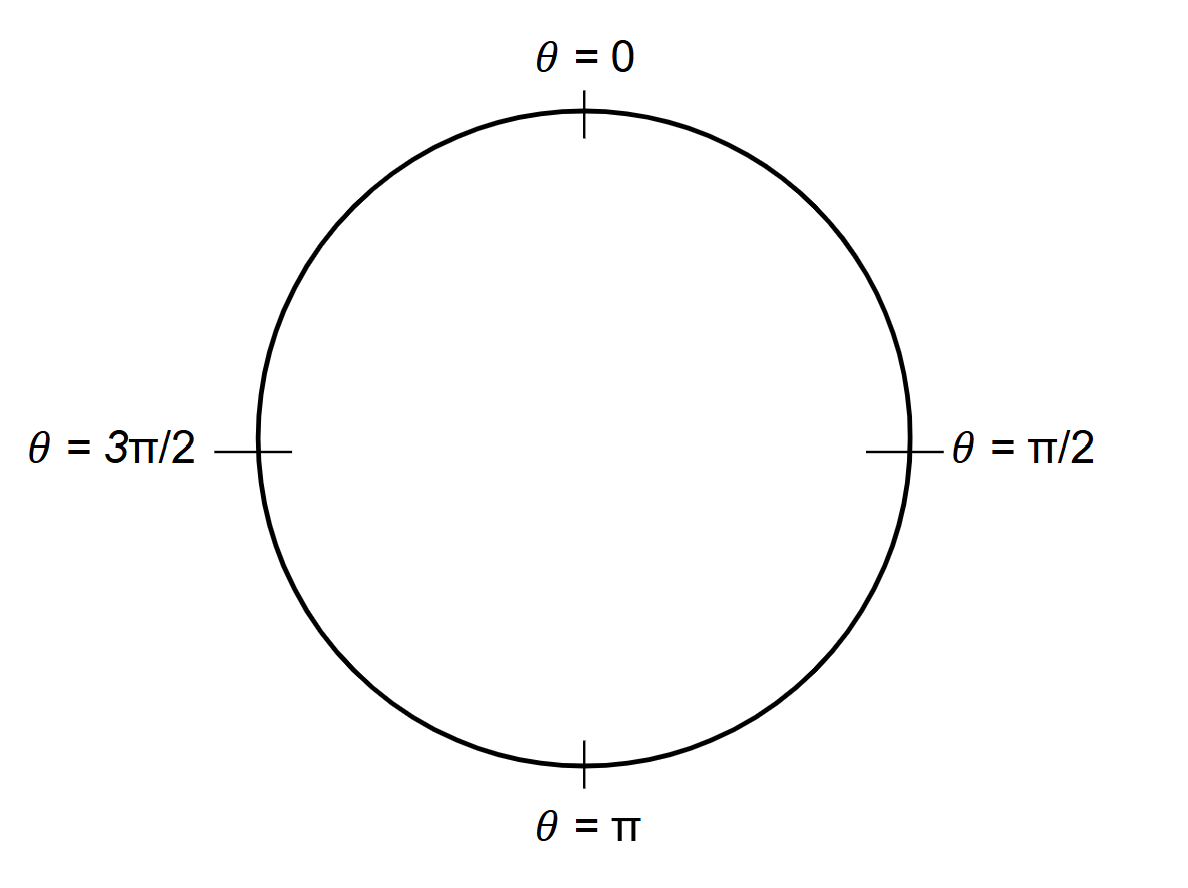
\includegraphics[width=\textwidth]{C:/Users/Matteo/Shallow-Water-Equations/figs/sphere1d_small_cell.png}
        \caption{Illustration of the grid for the 1D SWE with small cells.}\label{fig:sphere1d_small_cell}
    \end{subfigure}%
    \begin{subfigure}{0.35\textwidth}
        \centering
        \raisebox{10mm}{
        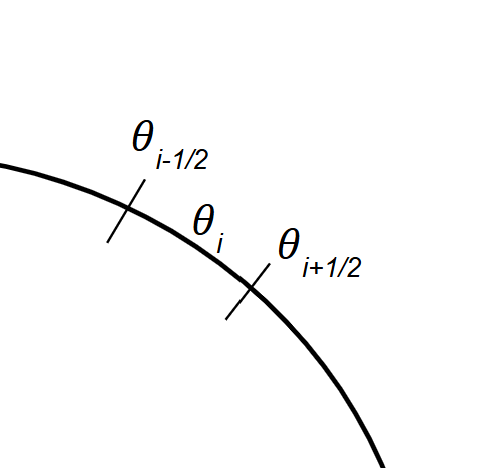
\includegraphics[width=0.9\textwidth]{C:/Users/Matteo/Shallow-Water-Equations/figs/sphere-1d-small-domain.png}
        }
        \caption{Illustration of the grid for the 1D SWE with a small domain.}\label{fig:sphere1d_small_domain}
    \end{subfigure}
    \caption{Grid illustrations for the 1D SWE in spherical coordinates.}\label{fig:sphere1d_combined}
\end{figure}
As when deriving the finite volume scheme for the 1D SWE in cartesian coordinates, we start by integrating the linearized shallow water equations over the control volume, and then divide by the cell length to obtain the finite volume scheme.
We integrate the vector form of the 1D SWE in spherical coordinates without the coriolis force over $\theta$ from $\theta_L := \theta_i - \frac{1}{2} \Delta \theta $ to $\theta_R := \theta_i + \frac{1}{2}\Delta \theta $ to obtain
\begin{align*}
    \int_{\theta_L}^{\theta_R} \mathbf{W}_t \text{ d}\theta + \int_{\theta_L}^{\theta_R} \mathbf{A} \mathbf{W}_\theta \text{ d}\theta = 0.
\end{align*}
Since the matrix $\mathbf{A}$ is constant, we can take it out of the integral:
\begin{align*}
    \int_{\theta_L}^{\theta_R} \mathbf{W}_t \text{ d}\theta + \mathbf{A} \int_{\theta_L}^{\theta_R} \mathbf{W}_\theta \text{ d}\theta = 0.
\end{align*}
We also use the fundamental theorem of calculus to rewrite the integral of the derivative as the difference of the function at the boundaries:
\begin{align}\label{eq:derive_integral_form_1D_spherical}
    \int_{\theta_L}^{\theta_R} \mathbf{W}_t \text{ d}\theta =  \mathbf{A} \left( \mathbf{W}(\theta_L, t) - \mathbf{W}(\theta_R, t) \right).
\end{align}
We can also write the equations out to get a better understanding of the terms:
\begin{equation}\label{eq:integral_form_spherical_1D}
    \left.
    \begin{aligned}
        \frac{\partial}{\partial t} \int_{\theta_L}^{\theta_R} h \text{ d}\theta + \frac{H}{r \cos(\phi)} (u_R - u_L) &= 0, \\
        \frac{\partial}{\partial t} \int_{\theta_L}^{\theta_R} u \text{ d}\theta + g(h_R - h_L) + fu_i &= 0.
    \end{aligned}
    \right\}
\end{equation}
Then we integrate~\eqref{eq:derive_integral_form_1D_spherical} over time from $t_1 := t_n$ to $t_2 := t_{n+1}$:
\begin{align*}
    \int_{t_1}^{t_2} \int_{\theta_L}^{\theta_R} \mathbf{W}_t \text{ d}\theta \text{ d}t = \mathbf{A} \left( \int_{t_1}^{t_2} \mathbf{W}(\theta_L, t) \text{ d}t - \int_{t_1}^{t_2} \mathbf{W}(\theta_R, t) \text{ d}t \right).
\end{align*}
Rewriting, using the fundamental theorem of calculus, gives
\begin{align}\label{eq:integral_form_spherical_1D_final}
    \int_{\theta_L}^{\theta_R} \mathbf{W}(\theta, t_2) \text{ d}\theta = \int_{\theta_L}^{\theta_R} \mathbf{W}(\theta, t_1) \text{ d}\theta
    - \mathbf{A} \left( \int_{t_1}^{t_2} \mathbf{W}(\theta_R, t) \text{ d}t - \int_{t_1}^{t_2} \mathbf{W}(\theta_L, t) \text{ d}t \right),
\end{align}
which we refer to as the integral form of the linearized shallow water equations in spherical coordinates with one spatial dimension and time.
We divide~\eqref{eq:integral_form_spherical_1D_final} with the cell length $\Delta \theta$ to obtain
\begin{align}
    \frac{1}{\Delta \theta} \int_{\theta_L}^{\theta_R} \mathbf{W}(\theta, t_2) \text{ d}\theta =
    \frac{1}{\Delta \theta} \int_{\theta_L}^{\theta_R} \mathbf{W}(\theta, t_1) \text{ d}\theta
    - \frac{\Delta t}{\Delta \theta} \mathbf{A} \left( \frac{1}{\Delta t} \int_{t_1}^{t_2} \mathbf{W}(\theta_L, t) \text{ d}t - \frac{1}{\Delta t} \int_{t_1}^{t_2} \mathbf{W}(\theta_R, t) \text{ d}t\right) .
\end{align}
Averaging over the terms for a finite volume $V_i^n$ gives the finite volume scheme for the linearized shallow water equations in spherical coordinates with one spatial dimension and time:
\begin{align}
    \mathbf{W}_i^{n+1} = \mathbf{W}_i^n - \frac{\Delta t}{\Delta \theta} (\mathbf{F}_{i+1/2}^n - \mathbf{F}_{i-1/2}^n),	
\end{align}
The FVM scheme can be written as 
\begin{align*}
    \mathbf{W}_i^{n+1} = \mathbf{W}_i^n - \frac{\Delta t}{\Delta \theta} (\mathbf{A}_{i+1/2}^n - \mathbf{A}_{i-1/2}^n) + \Delta t \mathbf{S}_i,
\end{align*}
where $\mathbf{W} = \begin{bmatrix} h \\ u \end{bmatrix}$, $\mathbf{A}_{i+1/2}^n$ is the numerical flux at the cell interface $\theta_{i+1/2}$, and $\mathbf{S} = \begin{bmatrix} 0 \\ fu \end{bmatrix}.$ 
With the cell averages:
\begin{align*}
    \mathbf{W}_i^{n} = \frac{1}{\Delta \theta} \int_{\theta_L}^{\theta_R} \mathbf{W}(\theta, t_1) \text{ d}\theta
\end{align*}
The flux $\mathbf{F}_{i-1/2}^n$ is the average flux across the line $\theta = \theta_{i-1/2}$ from time $t_n$ to $t_{n+1}$:
\begin{align*}
    \mathbf{F}_{i-1/2}^n = \frac{1}{\Delta t} \mathbf{A} \int_{t_1}^{t_{2}} (\mathbf{W}(\theta_L, t)) \text{ d}t,
\end{align*}
and correspondingly the flux $\mathbf{F}_{i+1/2}^n$ is the average flux across the line $\theta = \theta_{i+1/2}$ from time $t_n$ to $t_{n+1}$:
\begin{align*}
    \mathbf{F}_{i+1/2}^n = \frac{1}{\Delta t} \mathbf{A} \int_{t_1}^{t_{2}} (\mathbf{W}(\theta_R, t)) \text{ d}t.
\end{align*}

